\begin{figure}[!htb]
  \centering
  \begin{subfigure}[b]{0.3\textwidth}
    \centering
    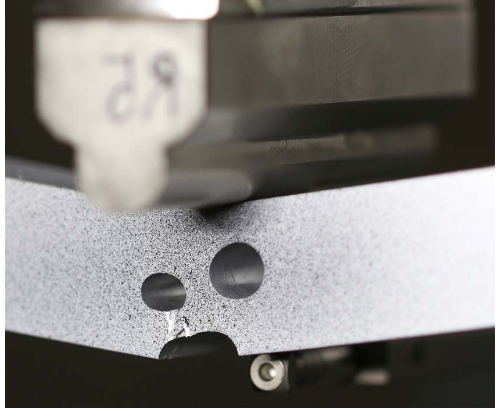
\includegraphics[width=\textwidth,scale=0.5]{Chapter5/figures/3pb/real_crack}
    \caption{}
  \end{subfigure}
  \hspace{0.1\textwidth}
  \begin{subfigure}[b]{0.35\textwidth}
    \centering
    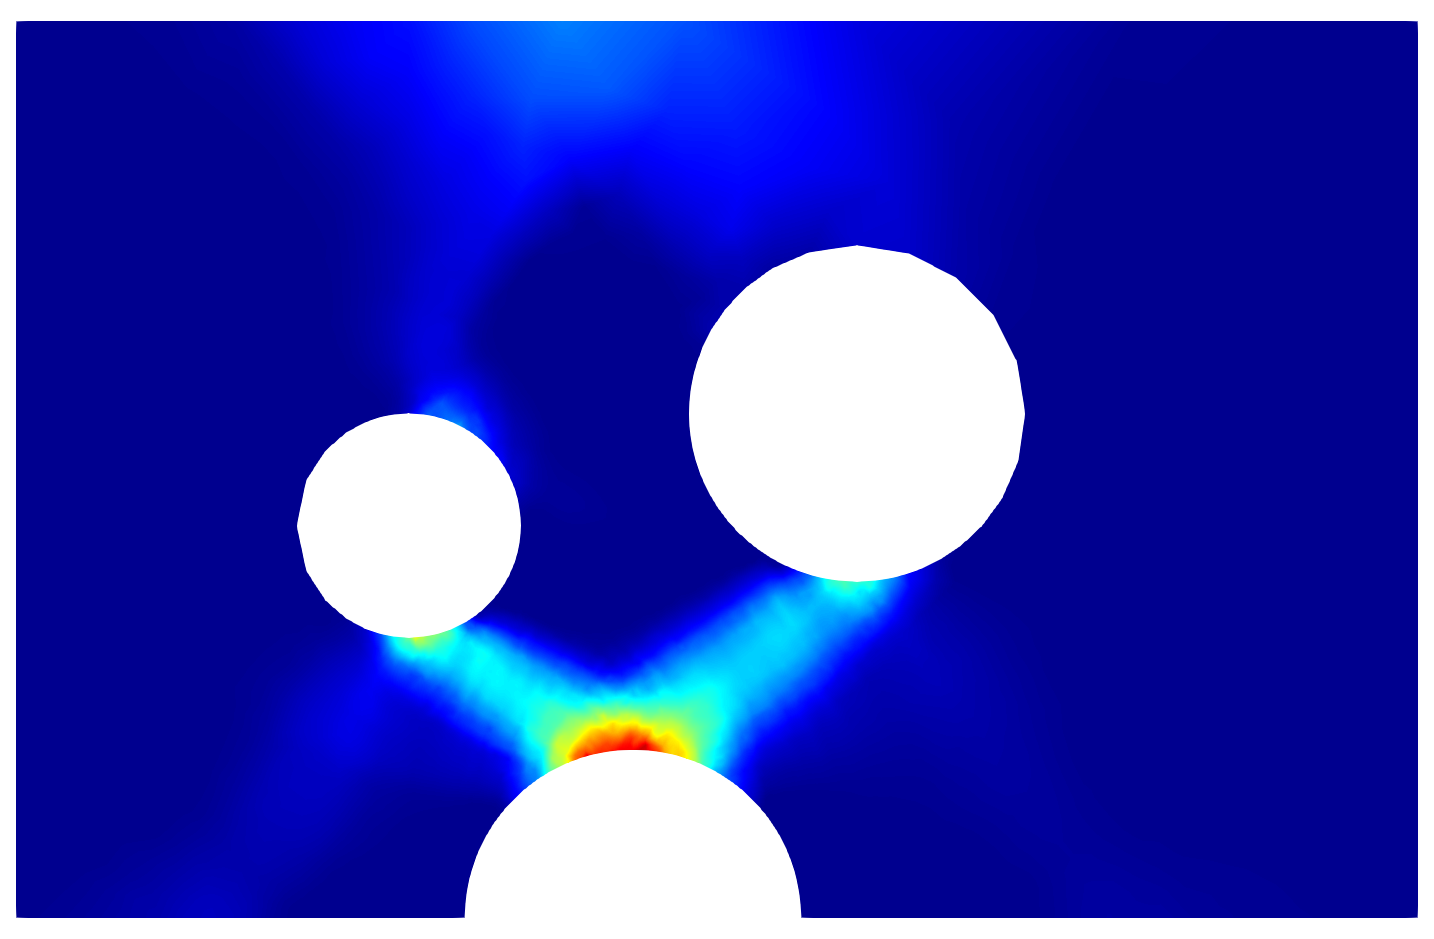
\includegraphics[width=\textwidth,scale=0.5]{Chapter5/figures/3pb/ep}
    \caption{}
  \end{subfigure}
  \begin{subfigure}[b]{0.06\textwidth}
    \centering
    \caption*{$\ep$}
    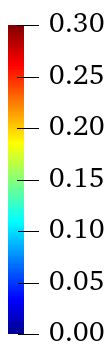
\includegraphics[width=\textwidth,scale=0.5]{Chapter5/figures/3pb/colorbar_ep}
    \vspace{1em}
  \end{subfigure}
  \label{fig: Chapter5/3pb/plastic_strain}
  \caption[A picture of the experiment setup and the effective plastic strain prior to crack initiation.]{(a) A picture of the experiment setup \cite{kubik2019ductile} and (b) the effective plastic strain prior to crack initiation. }
\end{figure}
